\section{Publish-Subscribe Subsystem}
\label{sec:ProcMngtSchedMain}

StreamFS uses a flexible construction of the publish/subscribe model in order to support a wide range of applications.
It addresses point \ref{rt} in section~\ref{sec:shortcomings}.  It includes both the process manager and processing
features that support \emph{online analytical processing (OLAP)} processing features.
Publish/subscribe is necessary is physical data application development in order to scale in the number of supported
applications.  The publish/subscribe model used in StreamFS provides mechanisms that enable a flexible combination 
of space and time decoupling that enable StreamFS to support of a wide arrange of application requirements, as described by
Eugster et al.~\cite{eugster}.
Our pub/sub engine is also tightly coupled with the namespaces exposed to users, and this design choice allows an application
to control the space coupling between the publisher and the subscriber (similar to TIBCO~\cite{tibco}).  

\subsection{Space decoupling}
By its very design, space decoupling is achieved.  Publisher do not hold a reference to the subscriber and subscribers do not
hold references to publishers.  However, because of the coupling of a full pathname and an object, subscriptions to topics
expressed as a full pathname refer to the single publisher.  Since we maintain a one-to-one mapping between the
name and an object, only a single stream can fulfill the subscription request.  Space decoupling is achieved when the 
topic is generalized using the star operator in a a regular expression match.  For example, if the user specifies
to obtain all the feeds for \texttt{/soda/4F/*} then all the publishers that have a name that match that prefix will be fowarded
to the subscriber sink.  Space decoupling in achieved because the subscriber and the publishers are unknown.

\subsection{Time decoupling}
Time decoupling is achievable through the timeseries data store.  Publisher push data to StreamFS whether or not subscribers are
online.  Moreover, data may be received at the subscriber even if the publisher becomes disconnected.  Currently, subscribers do
not receive all information that was missed.  In order to achieve fill time-decoupling, we allow the subcription
target to enable or disable the option to buffer all missed readings for an associated subscription target, while the subscription
target it offline.

\subsection{Synchronization decoupling}
Sychronization decoupling is achieved by the publisher and subscribers through StreamFS.  Events are received out of sequence
from their arrival to StreamFS.  This is true even when the subscription target is a processing element.  The thread that buffers
incoming data for each processing element is seperate from the thread where the process is executed.



\subsection{Implementation Details}

\begin{figure}[h!] %htbp
\centering
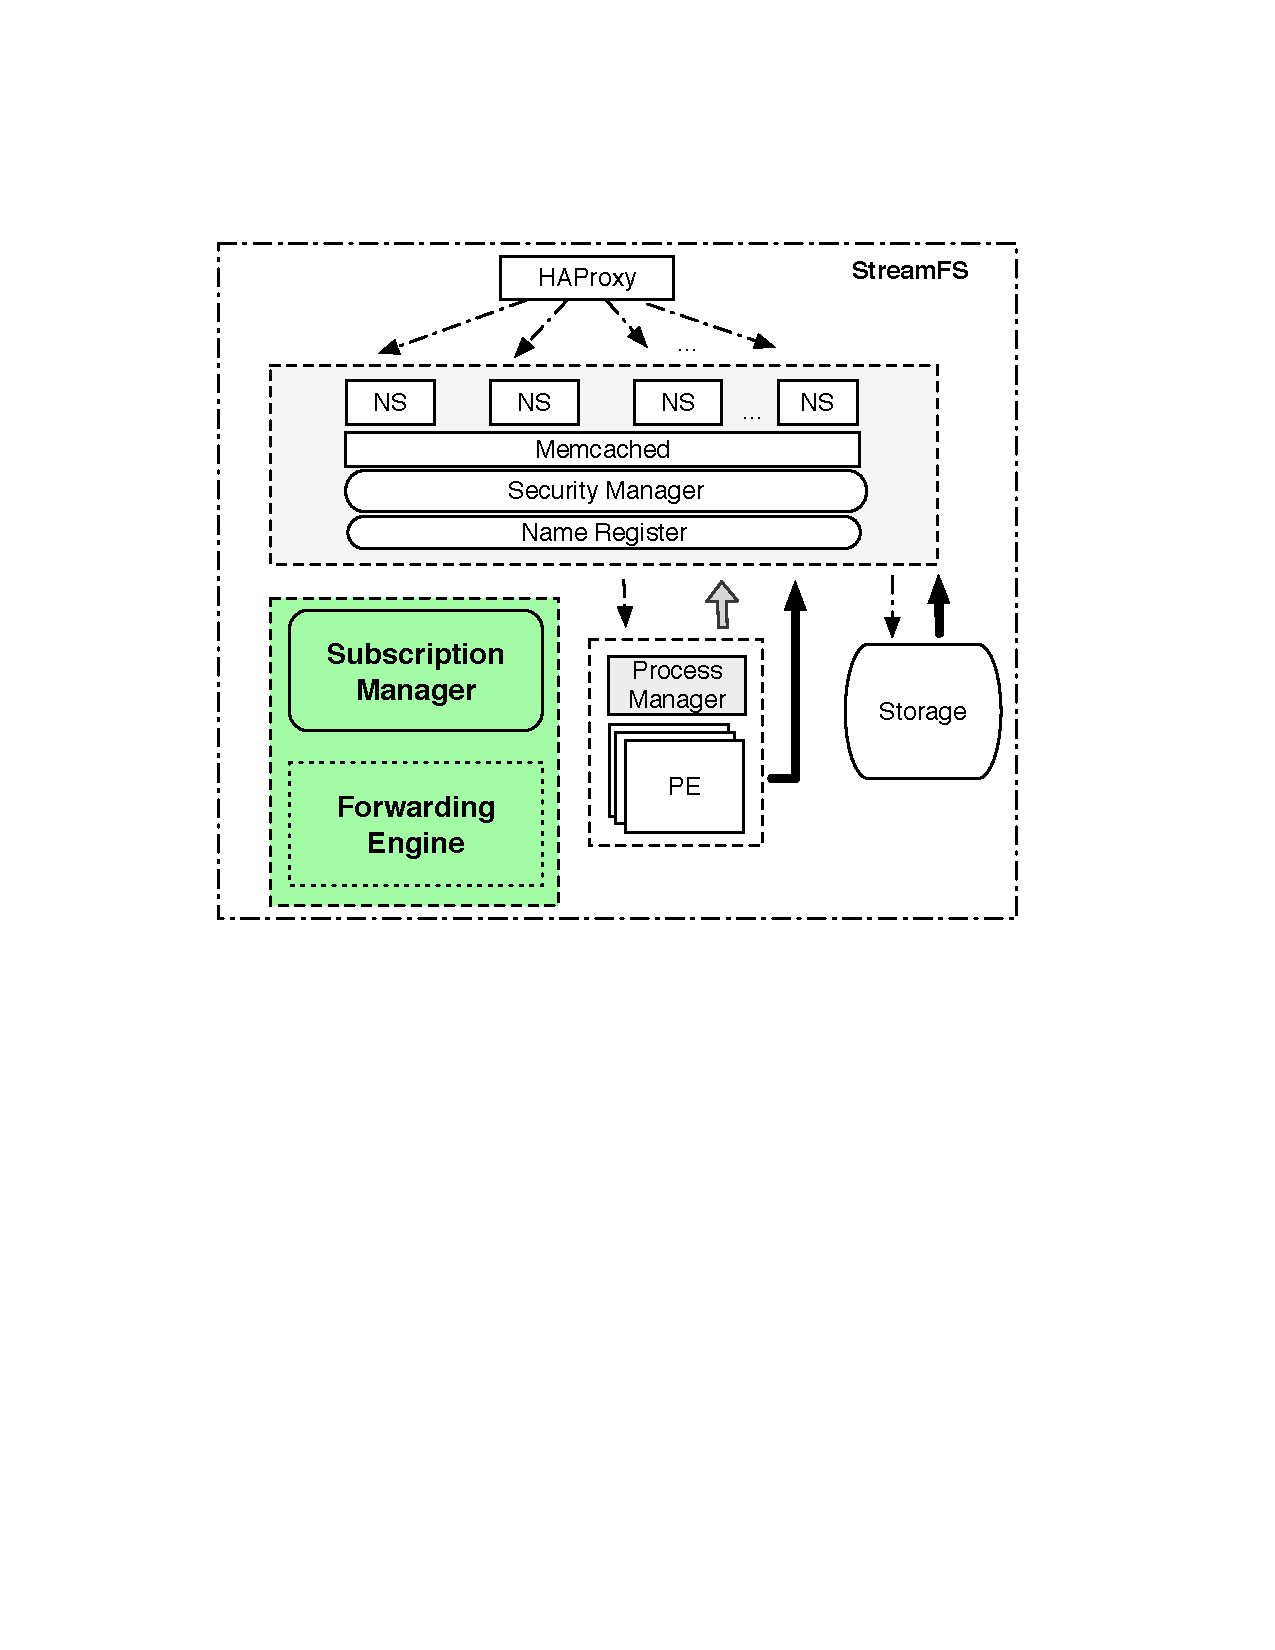
\includegraphics[width=.55\columnwidth]{figs/submngr}
\caption{}
\label{fig:submngr}
\end{figure}

The pub-sub system manager works with the name register to determine where to forward the incoming data.  When data arrives, it arrives
with a tag that contains the name of the publisher.  The subscription manager resolves the name to an object identifier and resolves
all the names for the object.  Then, it scans each of the names and matches them to a subscription.  If the subcription matches \emph{any}
name, the data unit is marked with the subscription id and sends to the forwarding engine.  The forwarding engine then
contact the forwarding sink and send it the data unit.  The subscription sink may be a processing element managed by the process manager.
If so, it is forwarded to the process manager's buffer and the process manager copies it to either an internal buffer for a
process that is running locally or sends it to an external process stub, which copies it in an internal buffer on the client side.